\def\year{2022}\relax
%File: formatting-instructions-latex-2022.tex
%release 2022.1
\documentclass[letterpaper]{article} % DO NOT CHANGE THIS
\usepackage{aaai22}  % DO NOT CHANGE THIS
\usepackage{times}  % DO NOT CHANGE THIS
\usepackage{helvet}  % DO NOT CHANGE THIS
\usepackage{courier}  % DO NOT CHANGE THIS
\usepackage[hyphens]{url}  % DO NOT CHANGE THIS
\usepackage{graphicx} % DO NOT CHANGE THIS
\urlstyle{rm} % DO NOT CHANGE THIS
\def\UrlFont{\rm}  % DO NOT CHANGE THIS
\usepackage{natbib}  % DO NOT CHANGE THIS AND DO NOT ADD ANY OPTIONS TO IT
\usepackage{caption} % DO NOT CHANGE THIS AND DO NOT ADD ANY OPTIONS TO IT
\DeclareCaptionStyle{ruled}{labelfont=normalfont,labelsep=colon,strut=off} % DO NOT CHANGE THIS
\frenchspacing  % DO NOT CHANGE THIS
\setlength{\pdfpagewidth}{8.5in}  % DO NOT CHANGE THIS
\setlength{\pdfpageheight}{11in}  % DO NOT CHANGE THIS
%
% These are recommended to typeset algorithms but not required. See the subsubsection on algorithms. Remove them if you don't have algorithms in your paper.
\usepackage{algorithm}
\usepackage{algorithmic}

\usepackage{tikz}
\usetikzlibrary {backgrounds, fit, calc} 
\usepackage{qcircuit}

%
% These are are recommended to typeset listings but not required. See the subsubsection on listing. Remove this block if you don't have listings in your paper.
\usepackage{newfloat}
\usepackage{listings}
\lstset{%
	basicstyle={\footnotesize\ttfamily},% footnotesize acceptable for monospace
	numbers=left,numberstyle=\footnotesize,xleftmargin=2em,% show line numbers, remove this entire line if you don't want the numbers.
	aboveskip=0pt,belowskip=0pt,%
	showstringspaces=false,tabsize=2,breaklines=true}
\floatstyle{ruled}
\newfloat{listing}{tb}{lst}{}
\floatname{listing}{Listing}
%
%\nocopyright
%
% PDF Info Is REQUIRED.
% For /Title, write your title in Mixed Case.
% Don't use accents or commands. Retain the parentheses.
% For /Author, add all authors within the parentheses,
% separated by commas. No accents, special characters
% or commands are allowed.
% Keep the /TemplateVersion tag as is
\pdfinfo{
/Title (AAAI Press Formatting Instructions for Authors Using LaTeX -- A Guide)
/Author (AAAI Press Staff, Pater Patel Schneider, Sunil Issar, J. Scott Penberthy, George Ferguson, Hans Guesgen, Francisco Cruz, Marc Pujol-Gonzalez)
/TemplateVersion (2022.1)
}

% DISALLOWED PACKAGES
% \usepackage{authblk} -- This package is specifically forbidden
% \usepackage{balance} -- This package is specifically forbidden
% \usepackage{color (if used in text)
% \usepackage{CJK} -- This package is specifically forbidden
% \usepackage{float} -- This package is specifically forbidden
% \usepackage{flushend} -- This package is specifically forbidden
% \usepackage{fontenc} -- This package is specifically forbidden
% \usepackage{fullpage} -- This package is specifically forbidden
% \usepackage{geometry} -- This package is specifically forbidden
% \usepackage{grffile} -- This package is specifically forbidden
% \usepackage{hyperref} -- This package is specifically forbidden
% \usepackage{navigator} -- This package is specifically forbidden
% (or any other package that embeds links such as navigator or hyperref)
% \indentfirst} -- This package is specifically forbidden
% \layout} -- This package is specifically forbidden
% \multicol} -- This package is specifically forbidden
% \nameref} -- This package is specifically forbidden
% \usepackage{savetrees} -- This package is specifically forbidden
% \usepackage{setspace} -- This package is specifically forbidden
% \usepackage{stfloats} -- This package is specifically forbidden
% \usepackage{tabu} -- This package is specifically forbidden
% \usepackage{titlesec} -- This package is specifically forbidden
% \usepackage{tocbibind} -- This package is specifically forbidden
% \usepackage{ulem} -- This package is specifically forbidden
% \usepackage{wrapfig} -- This package is specifically forbidden
% DISALLOWED COMMANDS
% \nocopyright -- Your paper will not be published if you use this command
% \addtolength -- This command may not be used
% \balance -- This command may not be used
% \baselinestretch -- Your paper will not be published if you use this command
% \clearpage -- No page breaks of any kind may be used for the final version of your paper
% \columnsep -- This command may not be used
% \newpage -- No page breaks of any kind may be used for the final version of your paper
% \pagebreak -- No page breaks of any kind may be used for the final version of your paperr
% \pagestyle -- This command may not be used
% \tiny -- This is not an acceptable font size.
% \vspace{- -- No negative value may be used in proximity of a caption, figure, table, section, subsection, subsubsection, or reference
% \vskip{- -- No negative value may be used to alter spacing above or below a caption, figure, table, section, subsection, subsubsection, or reference

\setcounter{secnumdepth}{0} %May be changed to 1 or 2 if section numbers are desired.

% The file aaai22.sty is the style file for AAAI Press
% proceedings, working notes, and technical reports.
%

% Title

% Your title must be in mixed case, not sentence case.
% That means all verbs (including short verbs like be, is, using,and go),
% nouns, adverbs, adjectives should be capitalized, including both words in hyphenated terms, while
% articles, conjunctions, and prepositions are lower case unless they
% directly follow a colon or long dash
\title{QNet: A Quantum-native Transformer Encoder Architecture}
\author{
    David Day,\textsuperscript{\rm 1}
}
\affiliations{
    %Afiliations
    \textsuperscript{\rm 1}Department of Computer Science Department & Information Engineering, National Central University\\
    % If you have multiple authors and multiple affiliations
    % use superscripts in text and roman font to identify them.
    % For example,

    % Sunil Issar, \textsuperscript{\rm 2}
    % J. Scott Penberthy, \textsuperscript{\rm 3}
    % George Ferguson,\textsuperscript{\rm 4}
    % Hans Guesgen, \textsuperscript{\rm 5}.
    % Note that the comma should be placed BEFORE the superscript for optimum readability

    2275 No. 300, Zhongda Rd.\\
    Taoyuan, Taiwan \\
    % email address must be in roman text type, not monospace or sans serif
    publications22@aaai.org
%
% See more examples next
}

% REMOVE THIS: bibentry
% This is only needed to show inline citations in the guidelines document. You should not need it and can safely delete it.
\usepackage{bibentry}
% END REMOVE bibentry
\usepackage[backend=bibtex,]{biblatex}
\addbibresource{references.bib}

\begin{document}

\maketitle

\begin{abstract}
AAAI creates proceedings, working notes, and technical reports directly from electronic source furnished by the authors. To ensure that all papers in the publication have a uniform appearance, authors must adhere to the following instructions.
\end{abstract}

\noindent 
\section{Introduction}

% Introduce quantum machine learning
Utilizing quantum computer on machine learning is a challenging task. Other than the gradient vanishing or exploding problem that already exists in classical computer, in the NISQ devices the qubits will incur decoherence after a long period of time. In addition, by the time that quantum computer is still developing, the quantum computing resource is limited. Researchers have to propose quantum machine learning model that can be verified on the current stage of NISQ and extensible for the large scale NISQ devices in the future.

% Introduce Transformer
Among various machine learning algorithms, the Transformer architecture family has achieved rapid and widespread dominance in various tasks, especially the models that use Transformer Encoder as its main component, for example, BERT-based model and Vision Transformer. Each block in the Transformer Encoder is composed of self Multi-head self-attention and Feedforward layer. The former is an inductive bias that connects each token in the input through a relevance weighted basis of every other token, and the latter is a linear transformation on each token.

% Introduce the problem -> large training cost (memory and time)
The one crucial shortcoming of Transformer is the time complexity of Multi-head attention. It performs matrix multiplication operation that needs time complexity of $O(n^2 \cdot d)$ to relate the tokens. This defect makes the time cost of directly input the long sequence to the model unacceptable. Multiple works~\cite{} have attempted to improve the performance of the Transformer Encoder, and most of them need to exchange accuracy with the speed.

% Introduce the potential of quantum computer
On the other hand, the hardware technologies of quantum computer are getting mature, which makes quantum algorithm as a possible solution to reduce the training cost of neural networks. At the time this paper is written, the quantum computer with 127 qubits was revealed~\cite{}. However, the actual capability of Quantum Machine Learning (QML) is still unknown. Multiple reports~\cite{} show that it indeed outperforms classical machine learning in certain situations. Most of the implementations of QML built on top of Variational Quantum Circuits (VQC), a promising class of algorithms that emerged as a central sub-field of QML. Based on VQC, multiple quantum Feedforward neural networks capable of universal quantum computation have been proposed~\cite{}, with the goal of using the potential of quantum computers in machine learning and attempting to train networks more effectively.

% Introduce the work.
In this work, we propose QNet, a novel sequence encoder model that entirely inferences on quantum computer. The architecture of the model is inspired by Transformer Encoder. The QNet reduces the inference time complexity while showing improvement on several tasks compared to other models.

% Show contribution, on XXXX datasets, the comparison
Two datasets, StackOverflow dataset and ColBERT dataset, are used to evaluation in the work. In the Stackoverflow dataset, QNet achieve accuracy 58.47 when embedding size is 2, while Transformer and FNet only reach 7.15 and 5.56 respectively. In the ColBERT dataset, with only 1 embedding dimension QNet can achieve accuracy 91.58 others need to have embedding dimension much larger than 1 to get to higher than 90. Therefore, we shows the quantum advantage on natural language processing tasks by using extremely small embedding dimension. 

% Show paper organization
This paper is organized to 7 sections. The introduction section points out the purpose of the work. The related work section shows the existing works that is related. The preliminary section brings in the required quantum computing knowledge. The method section describe the purposed model and the details of the work. The analysis section examine the time complexity of the model and compared with others. The experiments section verify the practicability of the work. In the last section, we conclude our work.


\section{Related Work}

\subsection{Transformer Architecture Family}

With the development of deep learning, Natural Language Processing (NLP) technology has become progressively mature.
Natural language processing refers to a technology that enables computers to analyze and understand human language, and human language has a sequence and context relationship. Recurrent Neural Network (RNN) is often used for such time series data. However, because RNN is difficult to perform parallel operations, Google proposed a network architecture that does not use RNN and CNN, but only a self-attention mechanism - Transformer~\cite{NIPS2017_3f5ee243}, in which each block is composed of Multi-head attention and a Feedforward layer. In recent years, it has achieved very good results in tasks such as sentiment analysis~\cite{naseem2020transformer}~\cite{wang2020transmodality}, machine translation~\cite{vaswani2018tensor2tensor}, speech recognition~\cite{dong2018speech},~\cite{gulati2020conformer} and dialogue robots~\cite{zandie2020emptransfo}~\cite{suglia2021embodied}.

The Transformer architecture has inspired multiple large scale NLP models. For instance, Generative Pretrained Transformer (GPT)~\cite{radford2019language}~\cite{NEURIPS2020_1457c0d6} is a new generation of learning language model released by OpenAI. GPT is based on the Transformer decoder. On the contrary, Bidirectional Encoder Representations from Transformers (BERT)~\cite{devlin2018bert} is mainly composed with a stack of Transformer encoder and a classification layer. BERT is a transformer-based machine learning technique for NLP pre-training developed by Google. It is designed to help computers understand the meaning of ambiguous language in text by using surrounding text to establish context.

The QNet in this work is isomorphic to Transformer Encoder, it can be said as a BERT related model.

\subsection{Attention-like Mechanism}

Recent works have shown the potential mathematics transformations that can replace Multi-head self-attention. The approach to replace self-attention with a transpose operation and a Feedforward layer has been proved to be able to achieve convincing results.

The work in~\cite{DBLP:journals/corr/abs-2105-02723} starts the question about the primitive property of attention mechanism. The work by \cite{DBLP:journals/corr/abs-2105-03824} shows that standard un-parameterized discrete Fourier transform can speed up Transformer encoder architectures, with limited accuracy costs, by replacing the self-attention sublayer with simple linear transformations that \emph{mix} input tokens.

\subsection{Quantum Neural Network}
By combining artificial neural networks with quantum computing principles, quantum neural networks have a strong potential to outperform classical neural networks. Quantum neural networks can process real-world data in addition to serving quantum data as the input.

Here, we concentrate on studies of quantum learning for an unidentified unitary transformation. \cite{PhysRevA.81.032324} specifically addressed this task and discovered an optimal method for storing and retrieving an unidentified unitary transformation on quantum memory. Soon after, \cite{PhysRevLett.122.170502} proposed an optimal unitary channel protocol that generalizes the results in~\cite{PhysRevA.81.032324}. In the most recent update, \cite{beer2020training} proposed a quantum neural network for learning an unidentified unitary quantum transformation that exhibits remarkable generalization behavior. 

Due to the small size of the experiment devices, we are unable to employ the quantum neural network model in this work. However, our work can theoretically be adapted to a quantum neural network by replacing the Variational Quantum Eigensolver circuit with a quantum Feedforward neural network. 

\subsection{Quantum Neural Networks For Sequential Input}

Sequential inputs are common to find in various tasks, for example, DNA sequence and NLP tasks. Recurrent Neural Networks and variants, for instance, Long Short-Term Memory~\cite{hochreiter1997long} and Gated Recurrent Units~\cite{cho2014learning}, dominate the tasks about sequential inputs before the Transformer architecture appears. Prior to this work, quantum implementation of recurrent neural networks~\cite{NEURIPS2020_0ec96be3} had been proposed. It is a model that is capable to inference fully on quantum computer. On the contrary, Quantum Long short-term memory~\cite{9747369} was also proposed. However, in the QLSTM, quantum computing is only used to enhance the input data by transforming data via Variational Quantum Eigensolver.

\section{Preliminary}

This section introduces the required quantum computing knowledge.

Quantum machine learning is a category of machine learning that makes use of quantum computers. In other words, quantum machine learning utilizes the properties of qubits and quantum gates. Instead of building machine learning models that purely support quantum computer, models designed in quantum-classical hybrid structure are more common for NISQ devices. One of the reasons is that the input data is always stored on classical computer because the decoherence of quantum computer will corrupt the data. In quantum-classical hybrid models, the quantum computer is used to either provide the quantum data by extracting input features or employ a quantum machine learning algorithm as the classifier.

In this work, our model can be seen as a representation encoder. We pipe the output of QNet to a classical classifier. However, the model does not restrict to this method. It can directly connect to a quantum neural network classifier to make it a pure quantum model.

\subsection{Quantum Fourier Transform}
Quantum Fourier transform is the quantum implementation of the discrete Fourier transform over the amplitudes of a quantum state. It converts the amplitudes from time domain to frequency domain.

Similar to discrete Fourier transform, Quantum Fourier transform maps the quantum state from $|X\rangle = \sum_0^{N-1} x_j|j\rangle$ to $|Y\rangle = \sum_0^{N-1} y_k |k\rangle$ according to Equation~\ref{equ:qft}, where $\omega^{jk}_N = e^{2\pi i \frac{jk}{N}}$.

\begin{equation} \label{equ:qft}
y_k = \frac{1}{\sqrt{N}} \sum_0^{N-1} x_j \omega_N^{jk}
\end{equation}

Quantum Fourier transform can also be expressed by the unitary matrix as Equation~\ref{equ:qft_u} with $\omega$ defined the same as above.

\begin{equation} \label{equ:qft_u}
U_{QFT} = \frac{1}{\sqrt{N}} \sum_{j=0}^{N-1}  \sum_{k=0}^{N-1} \omega_{N}^{jk} |k\rangle \langle j|
\end{equation}

In this work, Quantum Fourier transform is used in the purposed attention-like mechanism called "Quanttention".

\subsection{Variational Quantum Eigensolver}

The Variational Quantum Eigensolver (VQE)~\cite{} is a quantum-classical hybrid algorithm that can provide solutions in regimes which lies beyond the research of conventional algorithms. It is a form of quantum circuits with configurable parameters that are tuned by a classical computer in an iterative manner. In Fig.~\ref{fig:vqe}, a single layer VQE with 4 qubits is presented. $\alpha, \beta, \gamma$ are sets of learnable parameters to rotate qubits in 3-axis. Rotation gates are usually followed by entanglement gates to let qubits interact with each other to exchange the information. The VQE is to find an optimal transformation in a set of unitary transformations, which depends on the design of the quantum circuit.

The VQE approach has been shown to be flexible in circuit depth and the presence of noises. Therefore, while there is still lack of quantum error correction and fault-tolerant quantum computation in the noisy intermediate-scale quantum (NISQ) devices, quantum machine learning methods driven by variational quantum circuits can circumvent the complex quantum flaws that exist in the current quantum devices.


\begin{figure}[htp]
  \centering
  \fbox{
    \Qcircuit @C=2em @R=.7em {
    & \gate{R(\alpha^1_1, \beta^1_1, \gamma^1_1)} & \ctrl{1} & \qw & \qw & \targ & \qw \\
    & \gate{R(\alpha^1_2, \beta^1_2, \gamma^1_2)} & \targ & \ctrl{1} & \qw & \qw & \qw \\
    & \gate{R(\alpha^1_3, \beta^1_3, \gamma^1_3)} & \qw & \targ & \ctrl{1} & \qw & \qw\\
    & \gate{R(\alpha^1_4, \beta^1_4, \gamma^1_4)} & \qw & \qw & \targ & \ctrl{-3} & \qw
    }
  }
  \caption{Single-Layer VQE with 4 quantum wires.}
  \label{fig:vqe}
\end{figure}

\section{Method}

\subsection{Problem Formulation}

The purpose of this paper is to design a learnable quantum circuit for quantum computers with a similar architecture to the Transformer Encoder, and to explore how much improvement such a model can achieve.
Sequence-to-sequence learning is about training models to convert sequences from one domain to sequences in another domain. Using sequence-to-sequence model as backbone can also adapt the model to other tasks, such as text classification and image classification.

The methods of this paper are proposed under the following assumption.
\begin{itemize}
  \item There is a concept processing unit called QPU (Quantum Processing Unit), which is a NISQ device that can is connected to a classical computer. QPU can compute any basic quantum rotation gate and entanglement gate in $O(1)$ time complexity.
  \item There is a limited number of qubits on the QPU, for example, 32 qubits on the QPU.
  \item The inputs of the model will have the same length or can be chopped and padded into the same length.
\end{itemize}

The challenge to build a sequence-to-sequence learning model on current NISQ device is that the model has to utilize low number of qubits and shallow circuit. The development of NISQ device has made rapid progress recently; in 2021, IBM released the “Eagle” quantum computer, which has 127 qubits, making it the largest quantum computer at the time. However, it is still difficult to fit a classical sequence-to-sequence machine learning model into the size of a quantum computer. Even if it can, there is no obvious advantage to train the model on a quantum computer. In this work, We aim to propose an NLP model that is optimized for quantum computer and experiment on the NISQ device that is currently available.

\subsection{Architecture}

\begin{figure}[htp!]
  \centering
    \tikzstyle{layer} = [draw, text centered, text width=14em, minimum height=2em, rounded corners]
    \tikzstyle{ffblock} = [layer, fill=cyan!30]
    \tikzstyle{attnblock} = [layer, fill=orange!30]
    \tikzstyle{measure} = [layer, fill=green!10]
    \tikzstyle{encode} = [layer, fill=red!20]
    \tikzstyle{params} = [layer, fill=red!20]
    \begin{tikzpicture}
        \node (output) [text centered, text width=14em] {Outputs};
        \node (measure) [measure] [below of=output] {Pauli-Z Measurement};
        \node (ffblock) [ffblock] [below of=measure] {Simplified Quantum Feedforward};
        \node (attn) [attnblock] [below of=ffblock] {Quanttention};
        \node (encode) [encode] [below of=attn] {Input Encoding};
        \node (parameters) [params] [below of=encode] {Parameters Layer};
        \node (input) [text centered, text width=14em] [below of=parameters] {Inputs};
        
        \begin{scope}[on background layer]
            \node [fill=cyan!20, rounded corners, fit={(encode) (attn) (ffblock) (measure) }] {};
            \node [fill=orange!20, rounded corners, fit={(input) (parameters)}] {};
            \node [fill=orange!20, rounded corners, fit={(output)}] {};
            \node [draw, densely dashed, rounded corners, fit={(attn) (ffblock)}, label={right:$\times N$}] {};
            
            \draw[->] (input) -- (parameters);
            \draw[->] (parameters) -- (encode);
            \draw[->] (encode) -- (attn);
            \draw[->] (attn) -- (ffblock);
            \draw[->] (ffblock) -- (measure);
            \draw[->] (measure) -- (output);
        \end{scope}
        
        \matrix [draw,above] at ($(output)+(0, 0.8)$) {
          \node [fill=orange!20, rounded corners, label=right:Classical Computer] {}; \\
          \node [fill=cyan!20, rounded corners, label=right:Quantum Computer] {}; \\
        };
    \end{tikzpicture}
  \caption{The QNet Encoder Block Architecture.}
  \label{fig:qnet-encoder}
\end{figure}

In this section, we will describe the concept of QNet and purpose a residual connected QNet (ResQNet) which use QNet as its main component.

The concept of QNet can be separated into 3 parts. First, the word embedding is encoded onto a quantum computer. Second, a learnable word vector transformation and a token mixing mechanism are applied repeatedly to learn the representation of the combination of words. Finally, the measurement is applied on every qubit to take the quantum state back to classical computer. Since the result will be a flattened tensor, it has to be reshaped back to the original input shape.

The concept of QNet is simple. However, the actual process of QNet encoder is more complex and shown in Fig.~\ref{fig:qnet-encoder}. The quantum circuit has to be constructed for quantum compute before the execution. The parameters of word embedding and learnable word vector transformation have to be coded onto the circuit. The Parameters Layer in the figure prepares the parameters needed by the quantum circuit. The Input Encoding layer in the figure maps the word embedding into each qubit. The Quanttention layer introduces the mechanism to relate each token with others. The Simplified Quantum Feedforward Layer performs learnable unitary transformation on each token. The Quanttention layer and Simplified Quantum Feedforward layer can be repeated multiple times to mix the tokens more evenly. The QNet is only used to generate encoded representation. We will still use classical neural network to project the result of QNet into output space. To take the quantum data back to the classical computer, the Pauli-Z observable is used to measure the computed qubits.

\begin{figure}[htp!]
  \centering
    \tikzstyle{layer} = [draw, text centered, text width=14em, minimum height=2em, rounded corners]
    \tikzstyle{denseblock} = [layer, fill=violet!10]
    \tikzstyle{outputblock} = [layer, fill=blue!10]
    \tikzstyle{qnet} = [layer, fill=green!10]
    \tikzstyle{encode} = [layer, fill=red!20]
    \begin{tikzpicture}
        \node (output) [outputblock] {Output Projection};
        \node (dense) [denseblock] [below of=output] {Linear};
        \node (add) [font=\Large] [below of=dense] {$\oplus$};
        \node (qnet) [qnet] [below of=add] {QNet Encoder};
        \node (begin) [] [below of=qnet] {};
        \node (encode) [encode] [below of=begin] {Embedding Layer};
        
        \begin{scope}[on background layer]
            \node [draw, densely dashed, rounded corners, fit={($(begin)-(3.5, 0.2)$) ($(add)+(3.5, 0.2)$)}, label={right:$\times N$}] {};
            \draw[->] (encode) -- (qnet);
            \draw[->] (qnet) -- (add);
            \draw[->] (add) -- (dense);
            \draw[->] (dense) -- (output);
            
            \draw[->] (begin) -- ($(begin)+(3,0)$) -- ($(add)+(3,0)$) -- (add);
        \end{scope}
        
    \end{tikzpicture}
  \caption{The ResQNet - the model architecture.}
  \label{fig:resqnet}
\end{figure}

The ResQNet is a model that is composed by multiple residual connected QNet blocks, as shown in Fig.~\ref{fig:resqnet}. It is a feasible model for NISQ device and temporary replacement of quantum-native residual neural network since residual neural network is hard to implement on NISQ.

The derivation and circuit design are introduced in details in the following sections.

\subsubsection{Word Embedding Quantum Encoding}
The goal of the word embedding model is to map each token in the corpus into a $d$-dimensional vector with each dimension representing at least one meaning, that is, $f: [d] \rightarrow R^d$. 

In Transformer, the word embedding is added with \emph{positional encoding}. It is to make use of positional information in the model. In this work, we do not add the positional encoding to the word embedding. Instead, we utilize the property of qubits as follows.

We use two axes of qubits to encode data into the quantum computer. Word embeddings are transformed to the volume of a qubit, that is, the angle on Pauli-X. Thus, the range of numbers in the word embedding layer will fall in $[0, 2\pi)$. The position of the word is encoded as the phase of the qubit, that is, the angle on Pauli-Z. The angle of position information ranges in $[0, \pi)$. The transformation can be described as Equation~\ref{equ:word_embedding}. In the equation, $x$ is the input token array, and the superscript denote the index of the token and the subscript denote the index of the embedding. $n$ is the length of the input sequence, $d$ is the embedding dimension. This method can be visualized via the Bloch sphere as shown in Fig.~\ref{fig:word-sphere}.

\begin{equation} \label{equ:word_embedding}
x \rightarrow |\psi_x\rangle = ( \prod_{i=1}^n \prod_{j=1}^d R_x( \frac{(i-1) \pi}{n} )R_z(x^i_j) ) |0\rangle
\end{equation}

\begin{figure}[htp!]
    \centering
    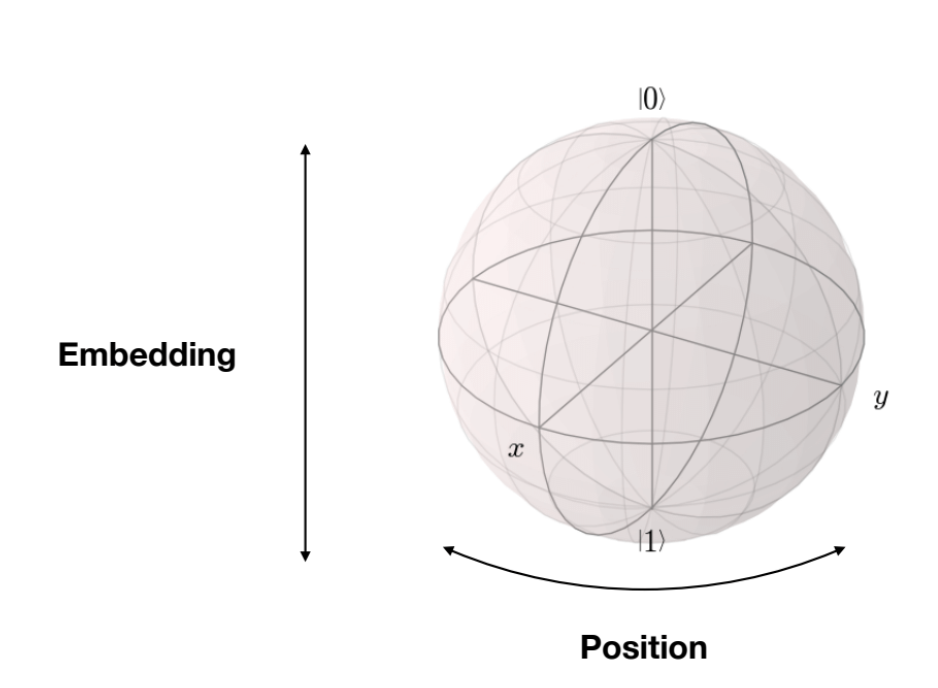
\includegraphics[width=7cm]{images/word-sphere.png}
    \caption{The Bloch sphere illustration of Word Embedding Quantum Encoding on a single qubit.}
    \label{fig:word-sphere}
\end{figure}

\begin{figure}[htp!]
  \centering
    \Qcircuit @C=2em @R=.7em {
    & |0 \rangle & & \gate{R_x(0)} & \gate{R_z(x^1_1)} & \qw & |\psi_1 \rangle & \\
    & |0 \rangle & & \gate{R_x(0)} & \gate{R_z(x^2_1)} & \qw & |\psi_1 \rangle & \\
    & |0 \rangle & & \gate{R_x(\frac{\pi}{2})} & \gate{R_z(x^1_2)} & \qw & |\psi_2 \rangle & \\
    & |0 \rangle & & \gate{R_x(\frac{\pi}{2})} & \gate{R_z(x^2_2)} & \qw & |\psi_2 \rangle & \\
    }
  \caption{The quantum circuit of Word Embedding Quantum Encoding for 2 words with 2 embedding.}
  \label{fig:embedding}
\end{figure}

\subsubsection{Quanttention}
A self-attention mechanism is an attempt to implement the action of selectively concentrating on a few relevant things, while ignoring others in deep neural networks~\cite{}.

In this work, we demonstrate why dot-product attention cannot be applied and propose a possible solution to implement the similar behavior. This solution considers the quantum computer resource on hand.

Since qubits are precious in the current stage NISQ, we do not want to use auxiliary qubits in this submodule. It is impractical to do the dot-product attention in the current scale of NISQ devices. For instance, the circuit of quantum state dot-product is shown in Fig.~\ref{fig:dot-product}. $\theta_1$ and $\theta_2$ are sets of learnable parameter for rotation gates in VQE. After the dot-product operation, $|\psi_1\rangle$ and $|\psi_2\rangle$ will be corrupted and cannot be recovered to the same state as before. Therefore, each time when the dot product is computed, the quantum state needs to be duplicated. There are at least $O(n \times d)$ dot-products, so this method is not feasible in the current NISQ device.

\begin{figure}[htp!]
  \centering
    \Qcircuit @C=2em @R=.7em {
    & |\psi_1 \rangle & & \gate{VQE(\theta_1)} & \qswap & \qw & \qw \\
    & |\psi_2 \rangle & & \gate{VQE(\theta_2)} & \qswap & \qw & \qw\\
    & |0\rangle & & \gate{H} & \ctrl{-2} & \gate{H} & \qw \\
    }
  \caption{The quantum circuit of Dot-Product with 2 quantum encoded word embedding.}
  \label{fig:dot-product}
\end{figure}


In FNet~\cite{}, the attention mechanism can be presented as Equation~\ref{equ:fnet}, in which $x$ is the input sentence while $F_h$ and $F_{seq}$ are Fast Fourier Transform on embedding dimension and sequence dimension, respectively. The results of FNet are approximately the same as the original multi-head attention.

\begin{equation} \label{equ:fnet}
y =  L_2(\mathbf{R}(F_{seq}(F_h(x))))
\end{equation}

If the purpose to perform the Fourier transform is just to \emph{mix} the tokens, the transformation can be simplified by removing the Fourier transform on the embedding dimension into Equation~\ref{equ:fnet-simple}.

\begin{equation} \label{equ:fnet-simple}
y = L_2(\mathbf{R}(F_{seq}(x)))
\end{equation}

By the concept of Equation~\ref{equ:fnet-simple}, we design the Quanttention mechanism. The unitary of Quantum Fourier Transform on the $i$-th embedding is presented in Equation~\ref{equ:u_qft}. In the equation, $n$ is the length of the input sentence and the $N$-th root of unitary is defined as $\omega^{jk}_N = e^{2\pi i \frac{jk}{N}}$.

\begin{equation} \label{equ:u_qft}
U_{QFT_i} = \frac{1}{\sqrt{n}} \sum_{j=0}^{n-1}  \sum_{k=0}^{n-1} \omega _{n}^{jk} |ki\rangle \langle ji|
\end{equation}

The Quanttention mechanism employs this unitary for each embedding. The formula is shown as Equation~\ref{equ:quanttention}. In the equation, $d$ is the embedding dimension.
 
\begin{equation} \label{equ:quanttention}
|y\rangle = U_{QFT_1}\ldots U_{QFT_d}|\psi\rangle
\end{equation}

Therefore, Quanttention is made up of Quantum Fourier Transforms performed on all tokens for each qubit in the embedding. The trainable quantum circuit is shown in Fig.~\ref{fig:quanttention}.

\begin{figure}[htp!]
  \centering
    \Qcircuit @C=2em @R=.7em {
    & |\psi^1_1 \rangle & & \qw & \multigate{1}{\ \mathcal{QFT}\ } & \qw & \qw \\
    & |\psi^2_1 \rangle & & \qswap & \ghost{\ \mathcal{QFT}\ } & \qswap & \qw \\
    & |\psi^1_2 \rangle & & \qswap \qwx & \multigate{1}{\ \mathcal{QFT}\ } & \qswap \qwx & \qw\\
    & |\psi^2_2 \rangle & & \qw & \ghost{\ \mathcal{QFT}\ } & \qw & \qw
    }
  \caption{Quanttention circuit.}
  \label{fig:quanttention}
\end{figure}


\subsubsection{Simplified Quantum Feedforward Network}

Quantum neural networks are known to have a three-dimensional architecture, with each neuron represented by a qubit. Because entanglement prevents the qubit from being reused, deep quantum neural networks are difficult to create with the existing NISQ technology.

Since the goal of this work is to construct a viable machine learning model, the Feedforward layer cannot include auxiliary qubits. Hence, the quantum neural network must be simplified. The circuit is shown in Fig.~\ref{fig:feedforward}

\begin{figure}[htp!]
  \centering
    \Qcircuit @C=2em @R=.7em {
    & |\psi^1_1 \rangle & & \multigate{1}{VQE(\theta_1)} & \multigate{1}{\ \mathcal{G}\ }& \multigate{1}{VQE(\theta_2)} & \qw \\
    & |\psi^2_1 \rangle & & \ghost{VQE(\theta_1)}& \ghost{\ \mathcal{G}\ } & \ghost{VQE(\theta_2)} & \qw \\
    }
  \caption{Simplified Quantum FeedForward with single vocab and 2 wires.}
  \label{fig:feedforward}
\end{figure}

In a typical transformer architecture, the Feedforward layer has two fully connected layers with one activation function between them. In the Simplified Quantum Feedforward layer, a similar arrangement is utilized, with two VQE separated by an activation function $\mathbf{G}$. The process can be demonstrated as Equation~\ref{equ:Feedforward}.

\begin{equation} \label{equ:Feedforward}
|\hat{\psi^1}\ldots\hat{\psi^m}\rangle = U_1U_\mathbf{G}U_2|\psi^1\rangle \ldots U_1U_\mathbf{G}U_2|\psi^m\rangle
\end{equation}

The objective of an activation function is to prevent gradient vanishing in a deep neural network model. It may be used millions of times, thus it must be computationally efficient.
The $\mathbf{G}$ is an amplitude amplification operator, which means that when the amplitude of a quantum state $|\psi\rangle = \sum^{2^{n}}_{i=1} x_i$ is described as $|x_i|^2$, the amplitude amplification operator will polarize the amplitudes. The unitary of $\mathbf{G}$ is expressed in Equation~\ref{equ:U_G}.

% Prove G operator by graph

\begin{equation} \label{equ:U_G}
U_\mathbf{G} = H^{\otimes m}(2|\psi\rangle\langle \psi|- I)H^{\otimes m}
\end{equation}

The circuit of $\mathbf{G}$ is shown in Fig.~\ref{fig:g-operator}.

\begin{figure}[htp!]
  \centering
    \Qcircuit @C=2em @R=.7em {
    & |\psi^1_1 \rangle & & \gate{H} & \ctrl{1} & \gate{H} & \qw \\
    & |\psi^2_1 \rangle & & \gate{H} & \ctrl{1} & \gate{H} & \qw \\
    & |\psi^3_1 \rangle & & \gate{H} & \targ & \gate{H} & \qw \\
    }
  \caption{Circuit of $\mathbf{G}$}
  \label{fig:g-operator}
\end{figure}

\subsubsection{Measurement}
In the end, quantum measurements on Pauli-Z are performed for every qubit. The measured result is a 1-D tensor with all entries lie in $[-1, 1]$. In order to pass the output into next block, that is, making the QNet as a sequence to sequence model. Tensor are shaped to the shape before entering the QNet.

\section{Model Analysis}

In this section, we examine the complexity of QNet and contrast it with Transformer encoder and FNet. On a classical computer, the complexity of a model is an asymptotic function of the number of basic arithmetic operations used. However, on a Quantum Computer, the time to execute the circuit is not the number of gates but equal to the depth of the circuit. The circuit depth is determined by observing the critical path, which is done by counting the dependent entanglement gates. In addition to the circuit depth, we also assess the gate complexity, which represents the asymptotic number of basic gates.

\begin{table}[htb!]
    \centering
    \begin{tabular}{ l|c|c  }
        \hline
        Circuit block & Gate Complexity & Circuit depth \\
        \hline
        Input Encoding & $O(n \cdot d)$ & $O(1)$ \\
        Quanttention &  $O(n^2 \cdot d)$ & $O(n)$ \\
        Feedforward &  $O(n \cdot d)$ & $O(d)$ \\
        \hline
    \end{tabular}
    \caption{Quantum circuit depth analysis of QNet, $n$ is the sequence length, $d$ is the representation dimension.}
    \label{table:depth}
\end{table}

In Table~\ref{table:depth}, the gate complexity and maximum circuit depth are computed.

In the input encoding, every qubit will have 2 rotation gates, but no entangle gate exists. Thus, the circuit depth is $O(1)$.
According to Theorem~2 in~\cite{892140} and the fact that there is no dependence on each Quantum Fourier Transform in Quanttention, the depth of Quanttention is $O(n)$.
In the Simplified Quantum Feedforward Network, we use the CNOT gate to entangle the neighboring qubit in the embedding dimension, so the depth of the circuit is the size of the embedding dimension $O(d)$.

\begin{table}[htb!]
    \centering
    \begin{tabular}{ l|c  }
        \hline
        Attention Type & Complexity\\
        \hline
        Quanttention & $O(n)$\\
        Self-Attention &  $O(n^2 \cdot d)$\\
        Fast Fourier Transform & $O(d \cdot  n \log n + n \cdot d \log d)$ \\
        \hline
    \end{tabular}
    \caption{Comparison of attention layer complexity, $n$ is the sequence length, $d$ is the representation dimension.}
    \label{table:attentions}
\end{table}

\begin{table}[htb!]
    \centering
    \begin{tabular}{ l|c  }
        \hline
        Feedforward Type & Complexity\\
        \hline
        Simplified Quantum Feedforward Network & $O(d)$ \\
        Positional-wised Feedforward Network &  $O(n \cdot d^2)$ \\
        \hline
    \end{tabular}
    \caption{Comparison of feedforward layer complexity, $n$ is the sequence length, $d$ is the representation dimension.}
    \label{table:feedforward}
\end{table}


In Table~\ref{table:attentions}, the Quanttention is compared with Self-Attention from Transformer and Fast Fourier Transform from FNet. In Table~\ref{table:feedforward}, the Simplified Quantum Feedforward Network is compared with Positional-Wised Feedforward Network. The Positional-Wised Feedforward Network is used in almost all the Transform based architecture, such as FNet. 

The model complexity is the addition of attention layer complexity and feedforward layer complexity. Based on Table~\ref{table:attentions} and Table~\ref{table:feedforward}, the overall model complexity is obtained as shown in Table~\ref{table:overval}.

\begin{table}[htb!]
    \centering
    \begin{tabular}{ l|c  }
        \hline
        Model & Overall Complexity \\
        \hline
        QNet & $O(n + d)$ \\
        Transformer &  $O(n^2 \cdot d + n \cdot d^2)$ \\
        FNet &  $O(d \cdot  n \log n + n \cdot d \log d + n \cdot d^2)$ \\
        \hline
    \end{tabular}
    \caption{Comparison of model overall operation complexity, $n$ is the sequence length, $d$ is the representation dimension.}
    \label{table:overval}
\end{table}

\begin{table*}[htb!]
    \centering
    \begin{tabular}{ |l|c|c|c|c|c|r|  }
        \hline
        Model & Epoch & Batch size & Embedding size & Num blocks & Initial LR & Accuracy \\
        \hline
        ResQNet & 5 & 128 & 1 & 1 & 0.0003 & \textbf{91.58} \\
        FNet & & & & & 1e-5 & 50.45 \\
        Transformer & & & & & & 50.45 \\
        \hline
        ResQNet & 5 & 128 & 2 & 1 & 0.0003 & \textbf{91.72} \\
        FNet & & & & & 1e-5 & 76.13 \\
        Transformer & & & & & & 86.59 \\
        \hline
        ResQNet & 5 & 128 & 3 & 1 & 0.0003 & \textbf{91.84} \\
        \hline
        FNet & 5 & 128 & 4 & 1 & 1e-5 & 90.83 \\
        Transformer & & & & & & \textbf{92.29} \\
        FNet & & & 8 & & & 91.99 \\
        \hline
    \end{tabular}
    \caption{The comparison of models when evaluating on ColBERT dataset.}
    \label{table:colbert_result}
\end{table*}

\begin{table*}[htb!]
    \centering
    \begin{tabular}{ |l|c|c|c|c|c|r|  }
        \hline
        Model & Epoch & Batch size & Embedding size & Num blocks & Initial LR & Accuracy \\
        \hline
        ResQNet & 5 & 128 & 1 & 1 & 0.0003 & \textbf{22.12}\\
        FNet & & & & & 1e-5 & 4.65\\
        Transformer & & & & & & 4.41\\
        \hline
        ResQNet & 5 & 128 & 2 & 1 & 0.0003 & \textbf{58.47} \\
        FNet & & & & & 1e-5 & 7.15 \\
        Transformer & & & & & & 5.56 \\
        Transformer & & & & 2 & & 6.35 \\
        Transformer & & & & 4 & 0.0003 & 6.53 \\
        \hline
        ResQNet & 5 & 128 & 3 & 1 & 0.0003 & \textbf{70.97} \\
        \hline
        FNet & 5 & 128 & 4 & 1 & 1e-5 & 24.00 \\
        Transformer & & & & & & 52.47 \\
        FNet & & & 8 & & & 48.68 \\
        Transformer & & & & & & \textbf{73.65} \\
        FNet & & & 16 & & & 71.18 \\
        \hline
    \end{tabular}
    \caption{The comparison of models when evaluating on Stackoverflow dataset.}
    \label{table:stackoverflow_result}
\end{table*}

\section{Experiments}

\subsection{Tasks}

In our experiments, we focus on natural language processing tasks that have short sequence input. The models are evaluated on classification task, regression task, and cross word task. All sentences are converted into lowercase and punctuation stripped. In addition, the consecutive tokens are separated by a white space. 

For text classification task, two datasets are used to evaluate the models, ColBERT~\cite{fw8e-z983-21} and StackOverflow~\cite{xu-etal-2015-short}. For review score prediction task, RentTheRunway~\cite{10.1145/3240323.3240398} dataset is used. For cross word task, Telomere-to-telomere~\cite{miga2020telomere} dataset is used. The descriptions of these datasets are as follows. % dataset and corresponding task

\subsubsection{Text Classification}
\begin{itemize}
  \item ColBERT dataset is a binary classification task for humor detection. It is consisted of 200,000 formal short texts (100,000 positive and 100,000 negative).
  \item StackOverflow dataset is a multi-class classification task to classify questions on StackOverflow.com. The data is consisted of randomly selected 20,000 question titles from 20 different tags (classes).
\end{itemize}

\subsubsection{Review Score Prediction}
RentTheRunway dataset is a regression task. The data are the measurements of clothing fit. We take review summary as input and predict the rating.

\subsubsection{Cross word}
Telomere-to-telomere dataset is human genome assembly. The input words are randomly masked, and the models have to predict the masked words.

The statistics of datasets are shown in Table~\ref{table:dataset-statistic}.

\begin{table}[htb!]
    \centering
    \begin{tabular}{ l|c|c|c|c  }
        \hline
        Dataset & Classes & Size & Length & $|V|$ \\
        \hline
        StackOverflow & 20 & 20,000 & 8.31/34 & 22,956 \\
        ColBERT & 2 & 200,000 & 12.81/22 & 74,010\\
        \hline
    \end{tabular}
    \caption{Statistics for the text datasets. Length (mean/max): the mean and max length of texts, and $|V|$: the vocabulary size.}
    \label{table:dataset-statistic}
\end{table}

\begin{table*}[htb!]
    \centering
    \begin{tabular}{ |l|c|c|c|c|c|r|  }
        \hline
        Model & Epoch & Batch size & Embedding size & Num blocks & Initial LR & Error \\
        \hline
        ResQNet & 5 & 128 & 1 & 1 & 0.0003 & \textbf{1.4865}\\
        FNet & & & & & 1e-5 & 2.0602 \\
        Transformer & & & & & & 2.0602 \\
        \hline
        ResQNet & 5 & 128 & 2 & 1 & 0.0003 & \textbf{1.4846} \\
        FNet & & & & & 1e-5 & 2.0654 \\
        Transformer & & & & & & 2.0603 \\
        % \hline
        % ResQNet & 5 & 128 & 3 & 1 & 0.0003 & \textbf{} \\
        \hline
        FNet & 5 & 128 & 4 & 1 & 1e-5 & 1.4516 \\
        Transformer & & & & & & \textbf{1.3773} \\
        \hline
    \end{tabular}
    \caption{The comparison of models when evaluating on RentTheRunway dataset.}
    \label{table:renttherunway}
\end{table*}

\subsection{Experimental Configuration}

This section describes the training regime to evaluate our models. We implemented the QNet with TensorFlow~\cite{abadi2016tensorflow}, a machine learning framework, and TensorFlow Quantum~\cite{broughton2020tensorflow}, a quantum machine learning library.
ResQNet is compared against Transformer and FNet under the common setting. Models are used as the backend for the same task. The learning rate is adjusted so that each model has the best validation accuracy.

\subsubsection{Hardware}

GPUs and TPUs are not used in the experiments due to the insufficient memory to simulate quantum computer. Instead, our model are trained distributed in supercomputer cluster, the Taiwania 1. In this work, 4 computing nodes are used, each node are equipped double 20 cores Intel Xeon Gold 6148 CPU and 384 GB RAM. To train the model in the cluster, the MultiWorkerMirroredStrategy of TensorFlow are used as the distribution strategy for synchronous training on multiple workers.

\subsubsection{Optimizer}

We used the Adam optimizer with $\beta_1 = 0.9$, $\beta_2 = 0.98$ and $\epsilon = 10^{-9}$.

In the distributed training environment, the loss of model is reduced to share cross multiple workers. Therefore, we have to adjust the learning rate according to batch size and number of nodes. The adjusted learning rate is defined as global learning rate in Equation \ref{equ:global_lr}.

\begin{equation} \label{equ:global_lr}
global\_lr = initial\_lr \times batch\_size \times num\_nodes
\end{equation}

We varied the learning rate over the course of training, according to the Cosine Decay strategy in Equation \ref{equ:lr}. In this work, $\alpha = 10^{-2}$.

\begin{equation} \label{equ:lr}
lr = global\_lr \times ( \frac{1}{2} (1 + cos( \frac{step}{total\_steps}\pi))(1 - \alpha) + \alpha)
\end{equation}

\subsection{Results}

\subsubsection{Text Classification}
For the text classification tasks, cross entropy are used to minimize the distance to the target. In specific, Categorical Cross Entropy loss is used for multi-class classification and Binary Cross Entropy for binary classification.

The configurations and results of ColBERT humor detection task are listed in Table~\ref{table:colbert_result}. As can be seen in the table, ResQNet achieves accuracy of 91.58\% with only 1 embedding dimension. Other models can only reach 90\% with more than 4 embedding dimensions.

The configurations and results of StackOverflow question classification task are listed in Table~\ref{table:stackoverflow_result}. As can be seen in the table, ResQNet outperforms other models more than 50\% in terms of accuracy when the embedding size is 2. Transformer needs embedding size of 4 to reach 52.47\% and FNet needs 8 embedding dimensions to reach 48.68\%. We tested multiple blocks with Transformer on embedding dimensions of 2, and it shows that the gap between ResQNet and Transformer is hard to close up using deeper neural networks.

\subsubsection{Review Score Prediction}
The review score prediction tasks are been viewed as regression tasks, so mean square error is used to optimize the model and as the evaluation metric on test data.

The configurations and results of the RentTheRunway review rating prediction task are listed in Table~\ref{table:renttherunway}. As can be observed in the table, ResQNet performs 0.57 lower error than other models with the embedding size of 2. 

\section{Conclusion}

\appendix
\printbibliography

\section{Acknowledgments}
AAAI is especially grateful to Peter Patel Schneider for his work in implementing the original aaai.sty file, liberally using the ideas of other style hackers, including Barbara Beeton. We also acknowledge with thanks the work of George Ferguson for his guide to using the style and BibTeX files --- which has been incorporated into this document --- and Hans Guesgen, who provided several timely modifications, as well as the many others who have, from time to time, sent in suggestions on improvements to the AAAI style. We are especially grateful to Francisco Cruz, Marc Pujol-Gonzalez, and Mico Loretan for the improvements to the Bib\TeX{} and \LaTeX{} files made in 2020.

The preparation of the \LaTeX{} and Bib\TeX{} files that implement these instructions was supported by Schlumberger Palo Alto Research, AT\&T Bell Laboratories, Morgan Kaufmann Publishers, The Live Oak Press, LLC, and AAAI Press. Bibliography style changes were added by Sunil Issar. \verb+\+pubnote was added by J. Scott Penberthy. George Ferguson added support for printing the AAAI copyright slug. Additional changes to aaai22.sty and aaai22.bst have been made by Francisco Cruz, Marc Pujol-Gonzalez, and Mico Loretan.

\bigskip
\noindent Thank you for reading these instructions carefully. We look forward to receiving your electronic files!

\end{document}
